% Figure 1: Experimental design schematic
\begin{figure}[htbp]
\centering
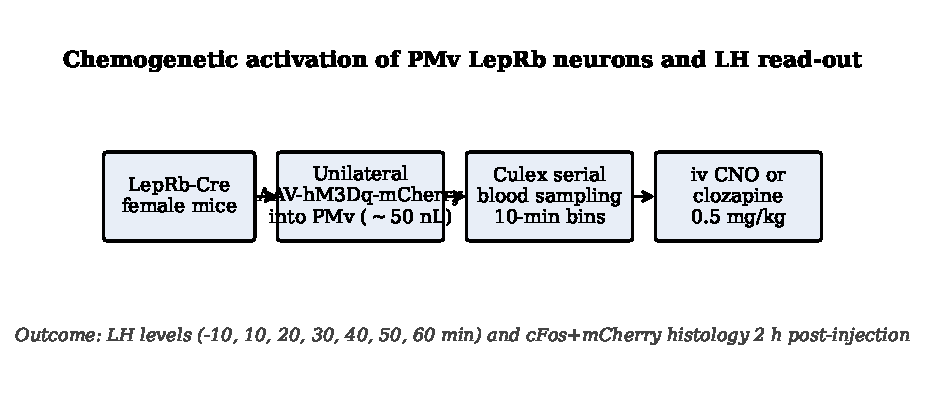
\includegraphics[width=0.95\textwidth]{figures/fig1_design.pdf}
\caption{Experimental design for chemogenetic activation of PMv LepRb neurons. Adult LepRb-Cre females (8--10 weeks) received unilateral stereotaxic injection of $\sim$50~nL of AAV-hM3Dq-mCherry into the ventral premammillary nucleus (PMv). Four weeks later, animals were connected to a Culex automated blood-sampling system; three baseline samples were drawn at 10-min intervals, and intravenous clozapine-$N$-oxide (CNO) or clozapine (0.5~mg/kg in 50~$\mu$L) was delivered at time 0. Serial LH measurements continued every 10 min for 60 min; brains were processed for cFos and mCherry immunofluorescence 2~h post-injection.}
\label{fig:design}
\end{figure}

% Figure 2: LH responder proportions
\begin{figure}[htbp]
\centering
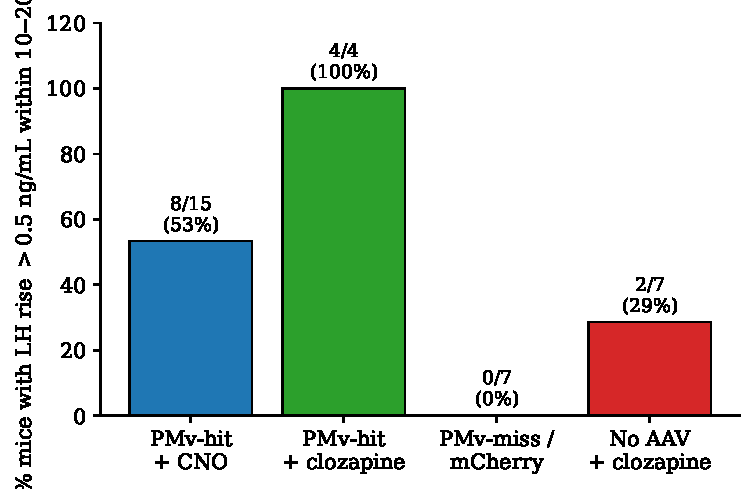
\includegraphics[width=0.7\textwidth]{figures/fig2_responders.pdf}
\caption{Proportion of mice with an LH rise greater than 0.5~ng/mL within 10--20 min of intravenous ligand injection, grouped by AAV targeting and ligand. 8/15 (55\%) of CNO-injected PMv-hit animals, 4/4 (100\%) of clozapine-injected PMv-hit animals, 0/7 of PMv-miss plus AAV-mCherry controls, and 2/7 (28.5\%) of no-AAV animals given clozapine alone responded. Absolute responder counts are printed above each bar.}
\label{fig:responders}
\end{figure}

% Figure 3: Estrous cycle count
\begin{figure}[htbp]
\centering
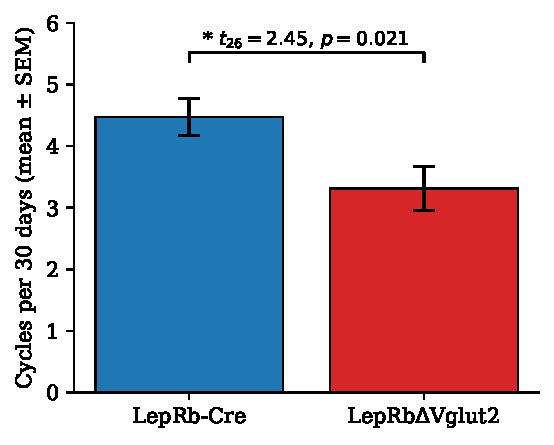
\includegraphics[width=0.5\textwidth]{figures/fig3_cycles.pdf}
\caption{Estrous cycles completed per 30 days in adult LepRb-Cre control ($4.47\pm0.30$) and LepRb$\Delta$Vglut2 ($3.31\pm0.36$) females. Bars show mean $\pm$ SEM; unpaired Student's $t$-test, $t_{26}=2.45$, $p=0.021$.}
\label{fig:cycles}
\end{figure}

% Figure 4: MBH qPCR
\begin{figure}[htbp]
\centering
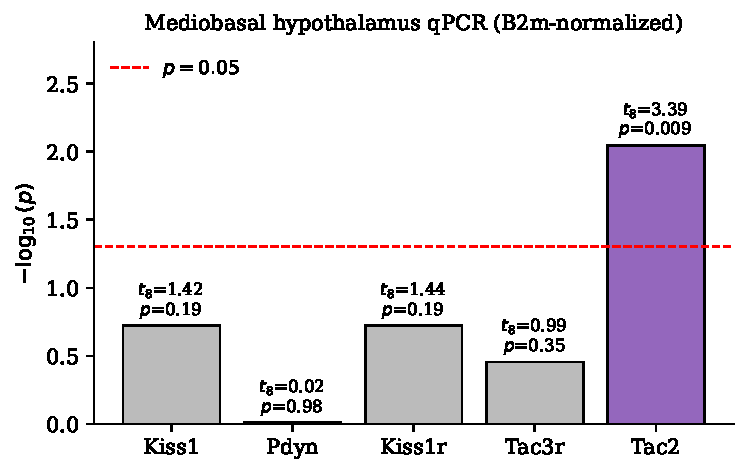
\includegraphics[width=0.75\textwidth]{figures/fig4_mbh_qpcr.pdf}
\caption{Mediobasal hypothalamic qPCR for KNDy-network transcripts in Vglut2$^{flox}$ ($n=5$) and LepRb$\Delta$Vglut2 ($n=5$) females, normalised to $\beta$-2-microglobulin. Bars show $-\log_{10}(p)$ for each comparison; dashed line marks $p=0.05$. Only Tac2 differed significantly between genotypes ($t_{8}=3.39$, $p=0.009$).}
\label{fig:mbhqpcr}
\end{figure}

% Figure 5: Working model
\begin{figure}[htbp]
\centering
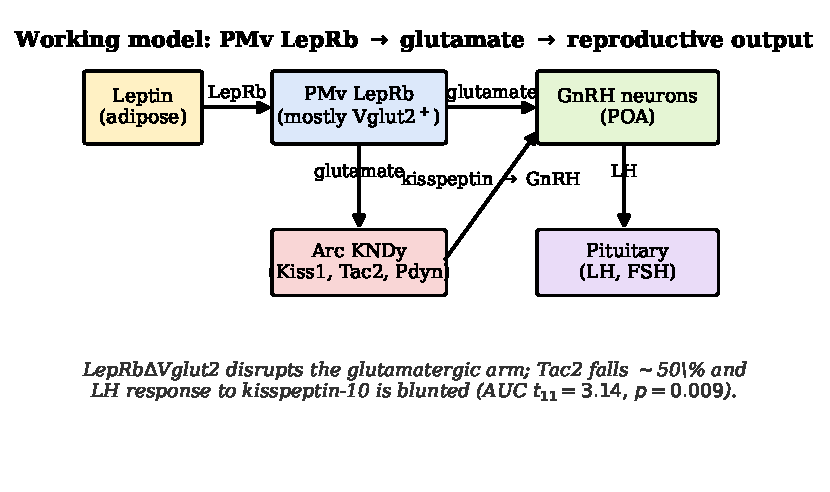
\includegraphics[width=0.85\textwidth]{figures/fig5_model.pdf}
\caption{Working model. Leptin acts on LepRb neurons of the PMv, most of which are glutamatergic (Vglut2$^{+}$). These neurons provide excitatory drive to GnRH neurons directly and, indirectly, to the Arc KNDy network through glutamate. In LepRb$\Delta$Vglut2 mice, the glutamatergic arm is disabled; downstream, hypothalamic Tac2 expression falls by $\sim$50\% and the LH response to exogenous kisspeptin-10 is blunted (AUC $t_{11}=3.14$, $p=0.009$).}
\label{fig:model}
\end{figure}

% Figure 6: Rescue experiment (qualitative ordinal)
\begin{figure}[htbp]
\centering
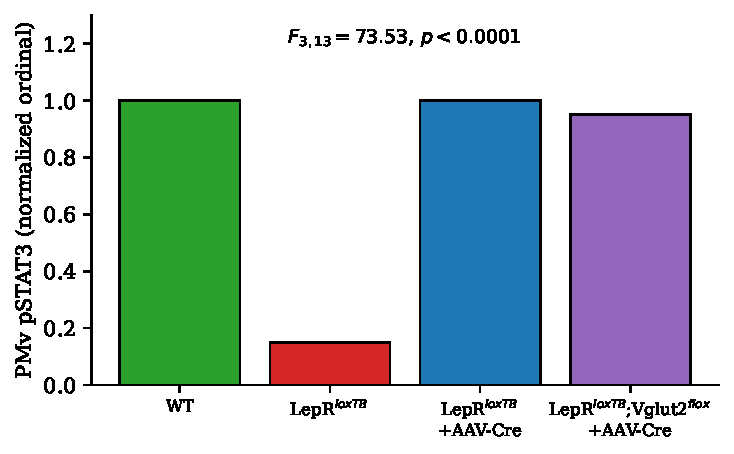
\includegraphics[width=0.7\textwidth]{figures/fig6_rescue.pdf}
\caption{Qualitative summary of leptin-induced pSTAT3 immunoreactivity in the PMv across the four groups of the rescue experiment: wild-type, LepR$^{loxTB}$ null, AAV-Cre-injected LepR$^{loxTB}$, and AAV-Cre-injected LepR$^{loxTB}$;Vglut2$^{flox}$. The ordinal bars indicate that PMv pSTAT3 is restored to wild-type levels by AAV-Cre in both genotypes, whereas it is essentially absent in uninjected LepR$^{loxTB}$ mice; overall one-way ANOVA $F_{3,13}=73.53$, $p<0.0001$. Despite restored LepR signalling, LepR$^{loxTB}$;Vglut2$^{flox}$ mice with correct PMv injections showed no vaginal opening or pregnancy.}
\label{fig:rescue}
\end{figure}
